\documentclass[12pt]{article}

\usepackage{listings}
\usepackage{cite}
\usepackage{graphicx}
\usepackage{color}
 
\definecolor{codegreen}{rgb}{0,0.6,0}
\definecolor{codegray}{rgb}{0.5,0.5,0.5}
\definecolor{codepurple}{rgb}{0.58,0,0.82}
\definecolor{backcolour}{rgb}{0.95,0.95,0.92}
\definecolor{codeblue}{rgb}{0.7,0.8,0.215}
 
\lstdefinestyle{newStyle}{
    backgroundcolor=\color{backcolour},   
    commentstyle=\color{codegreen},
    keywordstyle=\color{blue},
    numberstyle=\tiny\color{codegray},
    stringstyle=\color{codepurple},
    basicstyle=\footnotesize,
    breakatwhitespace=false,         
    breaklines=true,                 
    captionpos=b,                    
    keepspaces=true,                 
    numbers=left,                    
    numbersep=5pt,                  
    showspaces=false,                
    showstringspaces=false,
    showtabs=false,                  
    tabsize=2
}
 
\lstset{style=newstyle}

\usepackage[left=2cm,right=2cm,
    top=2cm,bottom=2cm,bindingoffset=0cm]{geometry}

\title{SOEN 6611 \\ SOFTWARE MEASUREMENT \\ Deliverable 1
(DESCRIPTIVE-STATISTICS)}
\date{SUMMER 2018}     
\author{(Team F)\\ 
Mehak Jot Kaur\\
Roopamdeep Kaur\\
Sukhmeet Kaur\\
Amandeep Kaur Khosa\\
Kritika Kritika\\
Dmitry Kryukov
}
%\setcounter{secnumdepth}{0}
\newcommand\tabularhead[1]{
\begin{table}[h]
  \caption{Use case - #1}
  \begin{tabular}{|p{0.35\linewidth}|p{0.65\linewidth}|}
    \hline
    \textbf{Use case name} & \textbf{#1} \\
    \hline}

  \newcommand\addrow[2]{#1 &#2\\ \hline}
  
  \newcommand\adddoublerow[2]{\begin{minipage}[t][][t]{2.5cm}#1\end{minipage}%
    &\begin{minipage}[t][][t]{\linewidth}
     \begin{itemize}\setlength{\itemsep}{0pt}%
        #2     
     \end{itemize}
     \end{minipage}\\ \hline}
  
  \newcommand\addmulrow[2]{ \begin{minipage}[t][][t]{2.5cm}#1\end{minipage}% 
     &\begin{minipage}[t][][t]{\linewidth}
      \begin{enumerate}\setlength{\itemsep}{0pt}%
        #2   
      \end{enumerate}
      \end{minipage}\\ \hline}
      
  \newenvironment{usecase}{\tabularhead}
{\hline\end{tabular}\end{table}}
% start of the document
\begin{document}            
\maketitle                  
\newpage
%-----------------------------------------------------------------
\section{Part - GQM}      
\subsection{Goal}

The goal of the descriptive-statistics project is to create a online school grading system to increase the efficiency of the studying process both for professors and students. The system will use descriptive statistics to show student grades, average grade, maximum grade, etc. Different actors will have different levels of access. Administrators can access every part of the statistical data and settings of the system and can't see the student related information. Students can see only their grades, average grade for the course, maximum and minimum grades, they have not access to the statistical data and other students grades. Professors have access to every part of the statistics and can edit this data if needed, see grades of all students, update grades.\cite{GQM} \cite{GQM-approach} \cite{GQM-wiki}

\subsection{Questions}

\begin{itemize}
   \item Question 1: How to understand that descriptive-statistics functions returns the correct results?\\
   Metric: Create a set of unit tests that will check the correctness of the results.
   \item Question 2: How to ensure that the student can get the grade less than 10 sec?\\
   Metric: Create a time-based tests to evaluate the time response of the system
   \item  How to ensure that the descriptive-statistics functions return results in less than 2 sec? \\
   Metric: Create a set of time-based unit tests to evaluate the speed of functions runtime.
   \item Question 4: How to ensure that the all users satisfied the online grading system?\\
   Metric: Create a quiz and collect the answers.
   \item Question 5: How to ensure that the system is effective for the students?\\
   Metric: Count the number of visits of the system per months by students.
   \item Question 6: How to ensure that the system is effective for the professors?\\
   Metric: Count the number of visits of the systems per month by professors.
   \item Question 7: What is inadequacy in the current working system?
   Metric: Calculate defect density.
   \item Question 8: How to ensure that the professors can update the any grade in the system in less than a minute?\\
   Metric: Create an integration test to test that action.
   \item Question 9: What are the bottlenecks of increasing effectiveness of the system?\\
   Metric: Time needed to do any action in the system.
   \item Question 10: How students can track their performance?
   Metric: By tracking metrics like GPA, rank in class, or 1st year performance in core subjects over time, they can identify both negative and positive patterns.
   \item Question 11: How much is the current reliability of the system?
   Metric: Mean Time to repair
   \item Question 12: What is the effectiveness level of testing process of system?
   Metric: Calculate defect removal efficiency.
   \item Question 13: What is current level of test coverage?
   Metric: Find number of failures.
   \item Question 14: How much people are needed to maintain this grading software ?
   Metric: Calculate assignment scope metric which will see how many people are needed to maintain this software and compare trends.


\end{itemize}
%-----------------------------------------------------------------
\section{Part - Use case model}
Use case model represent the interaction between actors and the system and shows the relationships between the actors and different use cases.\cite{UCM}
%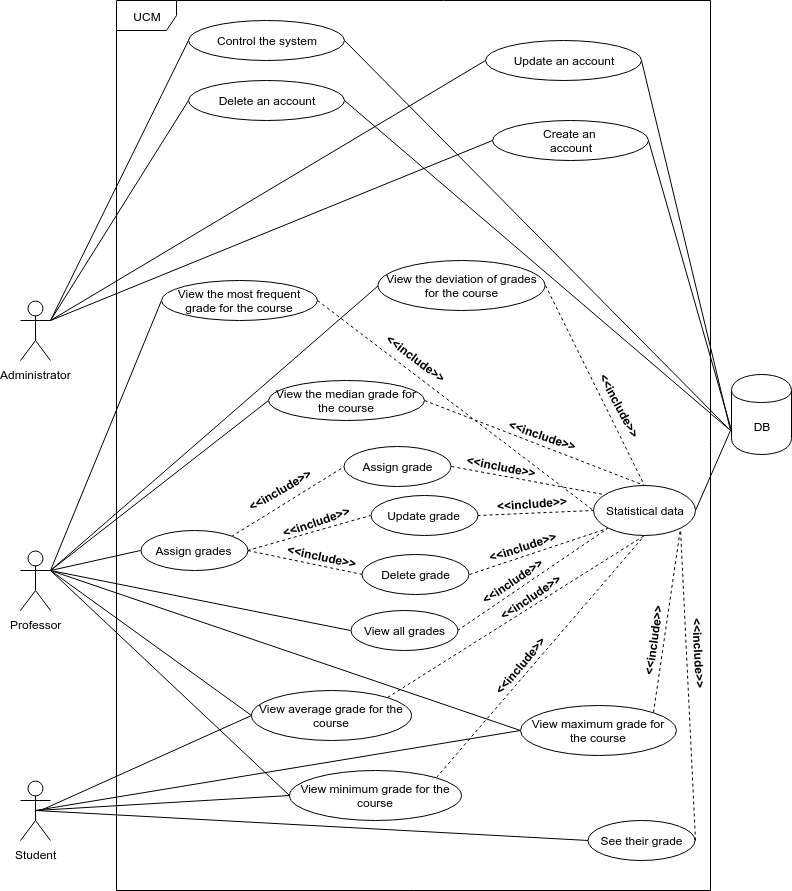
\includegraphics[width=\textwidth]{UCM.png}
\begin{figure}[h]
\centering
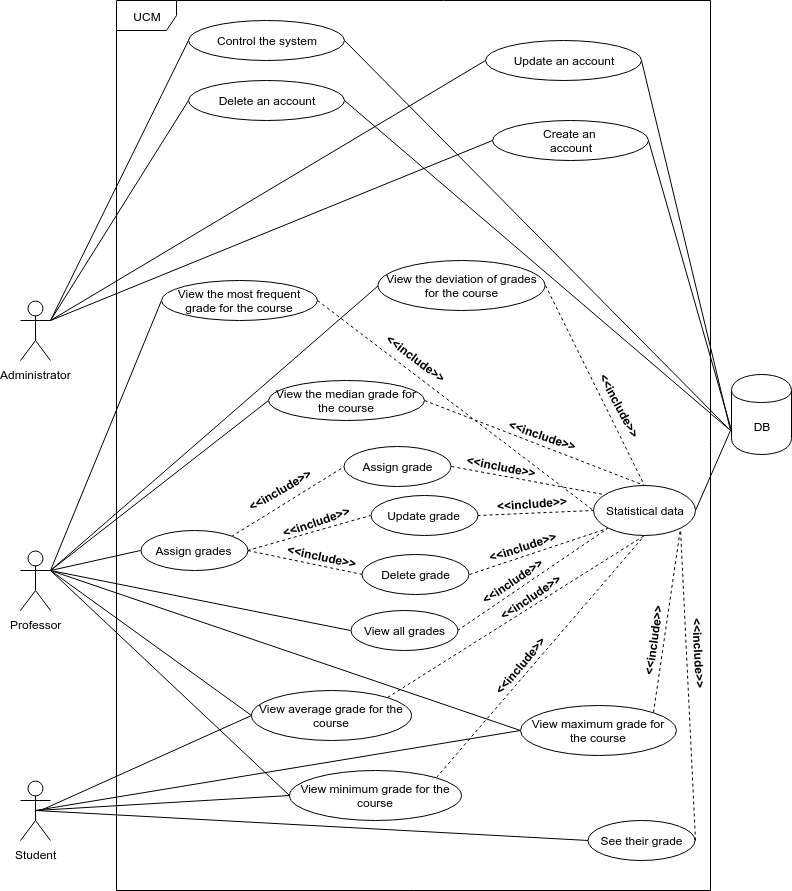
\includegraphics[width=0.8\textwidth]{UCM.png}
\caption{Use case model}
\end{figure}

\subsection{Use cases}
\begin{usecase}{Delete the grades}
    \addrow{Actors}{Professor}
    \addrow{Precondition}{Professor has access to the system}
    \addrow{Postcondition}{Professor deletes the grades.}
    \addmulrow{Main scenario (M)}{
        \item Professor login to the system
        \item System shows the list of available courses
        \item Professor chooses the desirable course
        \item System shows the list of students with its grades
        \item Professor chooses the student
        \item Professor delete the grade
    }
    \adddoublerow{Extensions (E)}{
        \item[] 1.1. Professor can't login
        \item[] 1.2. System suggest to contact to the Administrator
        \item[] 1.3. Go to 1
    }
\end{usecase}

\begin{usecase}{Update the grades}
    \addrow{Actors}{Professor}
    \addrow{Precondition}{Professor has access to the system}
    \addrow{Postcondition}{Professor updates the grades.}
    \addmulrow{Main scenario (M)}{
        \item Professor login to the system
        \item System shows the list of available courses
        \item Professor chooses the desirable course
        \item System shows the list of students with its grades
        \item Professor chooses the student
        \item Professor updates the grade
    }
    \adddoublerow{Extensions (E)}{
        \item[] 1.1. Professor can't login
        \item[] 1.2. System suggest to contact to the Administrator
        \item[] 1.3. Go to 1
    }
\end{usecase}
\newpage
\begin{usecase}{View all grades}
    \addrow{Actors}{Professor}
    \addrow{Precondition}{Professor has access to the system}
    \addrow{Postcondition}{Professor gets the all grades.}
    \addmulrow{Main scenario (M)}{
        \item Professor login to the system
        \item System shows the list of available courses
        \item Professor chooses the desirable course
        \item Professor see the grades
    }
    \adddoublerow{Extensions (E)}{
        \item[] 1.1. Professor can't login
        \item[] 1.2. System suggest to contact to the Administrator
        \item[] 1.3. Go to 1
    }
\end{usecase}

\begin{usecase}{Assign the grades}
    \addrow{Actors}{Professor}
    \addrow{Precondition}{Professor has access to the system}
    \addrow{Postcondition}{Professor assigns the grades.}
    \addmulrow{Main scenario (M)}{
        \item Professor login to the system
        \item System shows the list of available courses
        \item Professor chooses the desirable course
        \item System shows the list of students with its grades
        \item Professor assigns the grade
    }
    \adddoublerow{Extensions (E)}{
        \item[] 1.1. Professor can't login
        \item[] 1.2. System suggest to contact to the Administrator
        \item[] 1.3. Go to 1
    }
\end{usecase}

%-----------------------------------------------------------------
\section{Part - Estimates of effort}
\subsection{UCP}
hello world
\subsection{COCOMO 81}
hello world
\subsection{Difference in estimates using UCP and COCOMO 81}
hello world
%-----------------------------------------------------------------
\section{Part - Implementation}
\subsection{Code listings}
The code listing of implemented functions.
\subsubsection{Min function}

\begin{lstlisting}[language=R]
min <- function(array){
  res <- 9999999999999999
  for(elem in array){
    if(elem < res){
      res <- elem
    }
  }
  return(res)
}
\end{lstlisting}

\subsubsection{Max function}

\begin{lstlisting}[language=R]
max <- function(array){
  res <- -9999999999999999
  for(elem in array){
    if(elem > res){
      res <- elem
    }
  }
  return(res)
}
\end{lstlisting}
\subsection{Testing}

%-----------------------------------------------------------------
\section{Part - Cyclomatic complexity}

%-----------------------------------------------------------------
\section{Part - Object-oriented metrics}

%-----------------------------------------------------------------
\section{Part - SLOC}

%-----------------------------------------------------------------
\section{{Part - Correlations}}

%-----------------------------------------------------------------
%Don't delete below
\bibliography{ref}{}
\bibliographystyle{plain}
\end{document}               % End of document.